\documentclass[11pt]{article}
\usepackage[a4paper,margin=2.3cm]{geometry}
\usepackage{amsmath,amssymb,amsthm,bm}
\usepackage{booktabs,array,tabularx}
\usepackage{xcolor}
\usepackage{graphicx}
\usepackage{tikz}
\usetikzlibrary{arrows.meta,positioning,fit}
\usepackage[colorlinks=true,linkcolor=blue!50!black,urlcolor=blue!50!black]{hyperref}
\usepackage{enumitem}
\setlist{nosep,leftmargin=1.4em}

\newcommand{\R}{\mathbb{R}}
\newcommand{\sat}{\operatorname{sat}}
\newcommand{\clip}{\operatorname{clip}}
\newcommand{\sdf}{\operatorname{sdf}}
\newcommand{\Safe}{\mathcal{S}}
\newcommand{\Base}{\mathcal{B}}
\newcommand{\CN}{\mathcal{C}_N}
\newtheorem*{remark}{Remark}

\title{Safe low-altitude strike among obstacles and pursuing chasers\\[2pt]
\large Method summary for the sparse arena (PS2-RL strike task)}
\author{Kim Jungwon (with Claude)}
\date{22 October 2026}

\begin{document}
\maketitle

\begin{abstract}
A quadrotor must strike a slowly moving target at low altitude, among tall obstacles and a chaser that pursues it.
The requirement is no contact at all, together with a high strike rate.
The method has two layers.
A \emph{safety filter} certifies every command by checking that a backup policy, started from the next state, can still reach a recoverable hover without leaving the safe set.
A \emph{striker} policy, a learned correction on a pursuit controller, is then trained \emph{through} the filter (PS2).
This note gives the equations and a plain-words explanation of every part, the sparse-arena results, and the two open design decisions:
the filter type (discrete filter with escape variants vs.\ minimal-correction backup CBF) and the base set.
\end{abstract}

\tableofcontents

%======================================================================
\section{Overview}

\begin{center}
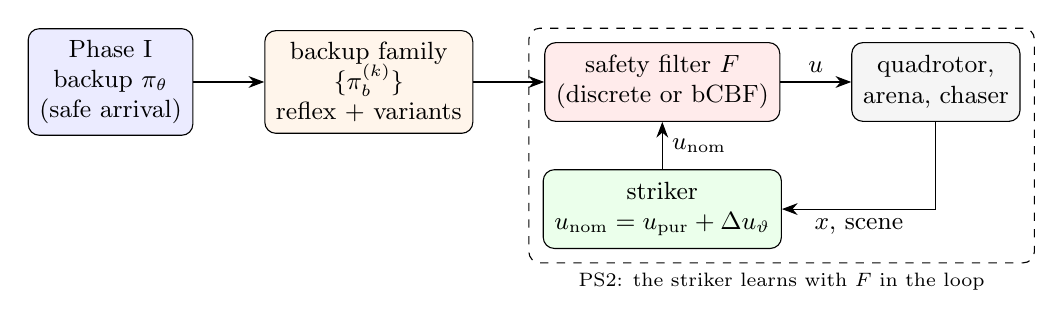
\begin{tikzpicture}[node distance=6mm and 9mm, every node/.style={font=\small},
  box/.style={draw, rounded corners, align=center, minimum height=10mm, inner sep=4pt, fill=#1!8}, box/.default=gray,
  >={Stealth[length=2mm]}]
\node[box=blue] (p1) {Phase I\\ backup $\pi_\theta$\\ (safe arrival)};
\node[box=orange, right=of p1] (fam) {backup family\\ $\{\pi_b^{(k)}\}$\\ reflex + variants};
\node[box=red, right=of fam] (filt) {safety filter $F$\\ (discrete or bCBF)};
\node[box=green, below=of filt] (str) {striker\\ $u_{\rm nom}=u_{\rm pur}+\Delta u_\vartheta$};
\node[box=gray, right=of filt] (plant) {quadrotor,\\ arena, chaser};
\draw[->] (p1) -- (fam);
\draw[->] (fam) -- (filt);
\draw[->] (str) -- node[right]{$u_{\rm nom}$} (filt);
\draw[->] (filt) -- node[above]{$u$} (plant);
\draw[->] (plant) |- node[pos=0.75,below]{$x$, scene} (str);
\node[draw, dashed, rounded corners, fit=(filt)(str)(plant), inner sep=5pt, label={[font=\scriptsize]below:PS2: the striker learns with $F$ in the loop}] {};
\end{tikzpicture}
\end{center}

\begin{enumerate}
\item \textbf{Safe set $\Safe$} (\S\ref{sec:safe}): no floor, obstacle, wall or ceiling contact; enough range to the chaser to still escape it (guidance-law margin $h_c$).
\item \textbf{Base set $\Base$} (\S\ref{sec:base}): hovering states whose hover ellipsoid is clear of everything; certified invariant under a hover LQR.
\item \textbf{Backup} (\S\ref{sec:phase1}--\ref{sec:family}): learned safe-arrival policy (hover LQR plus a learned correction), blended with an evasion reflex; several escape variants form a family of backups.
\item \textbf{Filter} (\S\ref{sec:discrete}--\ref{sec:bcbf}): keep the state inside the set from which some backup reaches $\Base$ within the horizon without leaving $\Safe$.
\item \textbf{Striker and PS2} (\S\ref{sec:striker}--\ref{sec:ps2}): residual on a pursuit controller, trained with the filter in the loop so that it learns routes the filter lets through.
\end{enumerate}

%======================================================================
\section{Task and model}\label{sec:model}

\paragraph{Quadrotor.}
State $x=(p,v,q)\in\R^3\times\R^3\times S^3$ (position, velocity, attitude quaternion); input $u=(a,\omega)$, collective thrust acceleration and body rates.
Explicit Euler with $\Delta t=0.02$\,s:
\begin{equation}
p_{k+1}=p_k+\Delta t\,v_k,\qquad
v_{k+1}=v_k+\Delta t\,\big(a_k R(q_k)e_3-g e_3\big),\qquad
q_{k+1}=\frac{q_k+\tfrac{\Delta t}{2}\,q_k\otimes(0,\omega_k)}{\|\cdot\|},
\end{equation}
with the input box $a\in[0,4g]$, $\omega\in[-18,18]^3$\,rad/s.
In words: a thrust-and-body-rate model, the interface PX4 offboard control accepts.

\paragraph{Arena (sparse).}
$40\times20$\,m, floor $z_f=1$\,m, ceiling $z_{\max}=10$\,m; three tall obstacles (rounded rectangles in the horizontal plane);
one chaser of radius $r_c=0.4$\,m pursuing the drone at speed $\le v_c=2$\,m/s and acceleration $\le 2$\,m/s$^2$, pushed away from obstacles;
the target starts at $x\in[32,37]$\,m, $z\in[1.6,2.5]$\,m and drifts at 0.2--0.8\,m/s.
A strike is a distance below 0.6\,m. An episode ends at a strike, a contact, leaving the arena, or after 10\,s.
The test set is 128 scenes (seed 9001), the same for every method.

\paragraph{Obstacles.}
Obstacle $i$ has centre $c_i$, half sizes $(b_x,b_y)$, yaw $\psi_i$ and rounding $r_i$ (a cylinder has $b=0$). With $\ell=R(\psi_i)^\top(p_{xy}-c_i)$,
\begin{equation}
\sdf_i(p_{xy})=\big\|\max(|\ell|-b,0)\big\|+\min\!\big(\max(|\ell_x|-b_x,|\ell_y|-b_y),0\big)-r_i,
\qquad \sdf_O=\min_i \sdf_i .
\end{equation}

%======================================================================
\section{Safe set}\label{sec:safe}

\begin{equation}
\Safe=\Big\{x:\ z-z_f\ge0,\ \ \sdf_O(p_{xy})\ge r_d,\ \ d_{\rm wall}(p_{xy})\ge r_d,\ \ z_{\max}-z\ge r_d,\ \ h_{c,j}(x)\ge 0\ \ \forall j\Big\},
\end{equation}
with drone radius $r_d=0.3$\,m. The first four terms are geometric. The last term is the chaser constraint, and it is where the design matters.

\subsection{Static reach ball (first version, rejected)}
Treat each chaser as a static obstacle of radius $R=r_c+r_d+v_cT$ ($=3.7$\,m for $T=1.5$\,s), i.e.\ everything it can reach within the backup horizon.
\textbf{Why it fails:} the ball is frozen at the chaser's current position, so it ignores where the chaser will be after $T$ and how fast the drone is closing on it.
A hover point chosen just outside the ball is reached by the chaser shortly afterwards.
Result: 49\,\% contacts with straight-line pursuit as the nominal (Table~\ref{tab:main}).

\subsection{Guidance-law escape margin (used)}
Let $R_j=\|p-c_j\|$ and $\hat e_j=(p-c_j)/R_j$ (line of sight from the chaser to the drone). The chaser closes the range at most at $v_c$, and the drone opens it at $\hat e_j^\top v$, so the worst-case closing speed is
\begin{equation}
s_j=v_c-\hat e_j^\top v,\qquad
h_{c,j}=R_j-(r_c+r_d)-s_j^+\,\delta-\frac{(s_j^+)^2}{2a_e},\qquad s^+=\max(s,0).
\end{equation}
\textbf{Meaning.} If the drone reacts after a lag $\delta$ and then raises its opening speed at $a_e$, it loses $s\delta+s^2/(2a_e)$ of range before it stops closing.
$h_c\ge0$ says that this distance is still available. We use $a_e=5$\,m/s$^2$, well below the vehicle's maximum, and $\delta=0.2$\,s.
\textbf{Required range:} 0.7\,m when flying away (at $\ge v_c$), 1.5\,m when hovering ($s=v_c$), 8.7\,m flying head-on at 6\,m/s ($s=8$).
In the GIFs the green dashed circle shows this required range.

\begin{remark}[Invariance in open space]
If the drone accelerates away along $\hat e$ at $a_e$ after the lag, then $\dot R\ge-s$ and $\dot s\le-a_e$, so
$\dot h_c\ge -s+a_e\delta+s=a_e\delta\ge0$ (up to line-of-sight rotation terms of order $v_c^2/(4R)$, covered by crediting $a_e$ below the true maximum).
So $\{h_c\ge0\}$ is invariant under ``flee'' when nothing blocks the way. Obstacles and walls are what can trap the drone, and that is why the filter has to check rollouts.
\end{remark}

%======================================================================
\section{Base set}\label{sec:base}

\paragraph{Hover LQR.}
Linearize about hover in $e=(p-a,\,v,\,\phi)$, with $\phi=2\,\mathrm{sgn}(q_w)\,q_{xyz}$ the small-angle attitude and $a$ a hover point.
Then take the discrete LQR of the Euler-discretized pair $(A_d,B_d)$ with weights $Q,R$: $P$ solves the DARE, $K=(R+B_d^\top PB_d)^{-1}B_d^\top PA_d$, and $V(e)=e^\top Pe$.

\paragraph{Re-anchoring (hover wherever the drone is).}
Write $r=(v,\phi)$ and split $P$ into position/rest blocks. The hover point minimizing $V$ is
\begin{equation}
a^\star(x)=p+Dr,\quad D=P_{pp}^{-1}P_{pr},\qquad
V_{\min}(r)=\min_a V=r^\top S r,\quad S=P_{rr}-P_{rp}P_{pp}^{-1}P_{pr}.
\end{equation}
The re-anchored LQR $u=u^\star-\tilde K r$, $\tilde K=K_r-K_pD$, brakes to a stop wherever the drone is.

\paragraph{Base set.}
\begin{equation}
\Base=\Big\{x:\ r^\top Sr\le c_B,\ \ \sdf_O(a^\star_{xy})\ge\rho_{xy}+r_d,\ \ a^\star_z-z_{\rm ext}\ge z_f,\ \ d_{\rm wall}(a^\star_{xy}),\ z_{\max}-a^\star_z\ \ge\rho_{xy}+r_d\Big\},
\end{equation}
where $\rho_{xy}=\sqrt{c_B\lambda_{\max}([P^{-1}]_{xy})}=1.22$\,m and $z_{\rm ext}=\sqrt{c_B[P^{-1}]_{zz}}=0.63$\,m are the extents of the hover ellipsoid $\{V\le c_B\}$ around $a^\star$.
\textbf{Meaning:} the drone is slow enough ($V_{\min}\le c_B$), and the whole region it can wander in while the hover LQR settles is clear of obstacles, floor and walls.

\paragraph{Certificate of $c_B$.}
Once the anchor is held fixed at $a_0$, the hover LQR $u=u^\star-K(p-a_0,r)$ keeps $V\le c_B$ (sublevel-set invariance), provided $c_B$ is below three bounds:
\begin{itemize}
\item $c_U=\min_i m_i^2/(K_iP^{-1}K_i^\top)$: the LQR command stays inside the input box on the ellipsoid;
\item $c_{\rm chart}=4/\lambda_{\max}([P^{-1}]_{\phi\phi})$: the attitude chart stays one-to-one;
\item $c_{\rm Lyap}$: a sampled one-step decrease $V^+/V<1$ of the nonlinear model on $\{V=c\}$, also under a worst-direction wind of 0.3\,m/s$^2$.
\end{itemize}
We use $c_B=50$, with $c_U=56.1$, $c_{\rm chart}=102.1$, $c_{\rm Lyap}=56.1$, and $V^+/V\le0.980$ (0.986 with wind).
Inside $\Base$ the level-flight speed is at most 2.67\,m/s and the tilt at most 52.7$^\circ$.

\paragraph{Hover latch.}
When a certified plan reaches $\Base$, the filter keeps that anchor $a_0$ and continues with the fixed-anchor LQR, which is the controller the certificate is about.
Re-anchoring at every step lets the anchor drift by millimetres, so a state that entered $\Base$ at zero margin drops out of it again.
Before the latch, 13 of 128 static scenes lost their certificate while hovering safely, and one of them then hit an obstacle.

\paragraph{Chasers and the base set (the open issue).}
No hover is invariant against a pursuer: wherever the drone stops, the chaser eventually arrives. The sparse-arena filter therefore keeps chasers \emph{out} of $\Base$ and handles them with
(i) the terminal condition $h_c\ge h_{\min}$ at the end of the certification rollout, and (ii) the evasion reflex inside the backup (\S\ref{sec:family}).
Alternatives are discussed in \S\ref{sec:decisions}.

%======================================================================
\section{Phase I: learned safe-arrival backup}\label{sec:phase1}

\paragraph{Policy.} A residual on the re-anchored hover LQR:
\begin{equation}
\pi_\theta(x)=\sat\big(u_{\rm LQR}(x)+\Delta u_\theta(o)\big),
\end{equation}
where the observation $o$ (98 numbers) contains $z-z_f$, $v$ and $q$; per obstacle slot (8, nearest first) the closest-point vector, centre offset, half sizes, $\cos2\psi$, $\sin2\psi$, rounding and presence; per chaser slot (2) the ball centre offset, radius and presence.
The slots keep the order they had at the rollout start, and membership in $\Safe$ and $\Base$ is an exact function of $o$.

\paragraph{Objective (safe arrival).} An episode is one backup rollout from a sampled (state, scene) pair:
\begin{equation}
\max_\theta\ \mathbb{E}\Big[\beta^{\tau_\Base}\,\mathbf 1\{\text{$\Base$ reached at $\tau_\Base$ before leaving $\Safe$}\}\Big],\qquad \beta=0.99,
\end{equation}
trained with TD3 and an anchor penalty $0.2\,\|\Delta u/u_{\rm scale}\|^2$ that keeps the residual small.
\textbf{Meaning:} reach a safe hover as fast as possible, and never leave the safe set on the way.
The backup is evaluated by membership in $\CN$: $\Base$ reached within $N=T/\Delta t$ steps ($T=1.5$\,s) without leaving $\Safe$.

\paragraph{Regions.} \emph{General} (random speed, tilt, scenes), \emph{blocked} (fast, with an obstacle where the LQR would stop), \emph{chaser} (fast, with a chaser ball where the LQR would stop), \emph{shell} (slow and near hover).
Mixture $(0.4,0.2,0.2,0.2)$, 5M steps (about 5 minutes on the GPU).

\begin{table}[h]\centering\small
\caption{Phase I, fraction in $\CN$ on held-out test scenes (2000 per region). The chaser here is a static ball (first version).}
\begin{tabular}{lccccc}\toprule
backup & general & blocked & chaser & shell & weighted\\\midrule
hover LQR (brake in place) & 0.556 & 0.001 & 0.079 & 1.000 & 0.438\\
learned (TD3, anchor 0.2) & \textbf{0.840} & \textbf{0.365} & \textbf{0.452} & 1.000 & \textbf{0.699}\\\bottomrule
\end{tabular}
\end{table}

%======================================================================
\section{Backup family used by the filter}\label{sec:family}

\paragraph{Composed backup.} The fixed-anchor hover LQR inside $\Base$, and $\pi_\theta$ outside it (the actor never trained inside $\Base$):
$u_{\rm base}(x)=u_{\rm hold}(x;a_0)$ if $x\in\Base$ (latched), else $\pi_\theta(x)$.

\paragraph{Evasion reflex.} With $h_{\min}(x)=\min_j h_{c,j}(x)$, the reflex weight is
\begin{equation}
\sigma(x)=\clip\!\Big(\frac{h_{\rm off}-h_{\min}(x)}{h_{\rm off}-h_{\rm on}},0,1\Big),\qquad h_{\rm on}=0.5\text{\,m},\ h_{\rm off}=2.0\text{\,m},
\end{equation}
and the backup command is the blend
\begin{equation}
\pi_b(x)=\sat\big((1-\sigma)\,u_{\rm base}(x)+\sigma\,u_{\rm esc}(x)\big).
\end{equation}
The escape command $u_{\rm esc}$ flies away from the most critical chaser, deflected by obstacles and walls near the hover point:
\begin{align}
d&=\mathrm{normalize}\Big(R(\theta)\,\hat e_{xy}+2\,\varpi_o\,n_o+2\textstyle\sum_w \varpi_w n_w\Big),\qquad
\varpi=\clip\!\Big(\frac{d_{\rm push}-(\text{dist}-\rho_{xy}-r_d)}{d_{\rm push}},0,1\Big),\\
v_{\rm des}&=\big(v_{\rm esc}\,d,\ 1.5\,(z_{\rm ref}-z)\big),\qquad z_{\rm ref}=\clip(z,\,z_f+1,\,z_{\max}-3),
\end{align}
where $n_o=\nabla\sdf_O$, $n_w$ are the wall normals, the distances are measured at the anchor, and $d_{\rm push}=1.5$\,m.
A velocity loop tracks $v_{\rm des}$: $a_{\rm des}=k_v(v_{\rm des}-v)$ (horizontal part limited to a 45$^\circ$ tilt) $+\,g e_3$, thrust $a=a_{\rm des}^\top z_b$, body rates $\omega=k_{\rm att}R^\top(z_b\times\hat a_{\rm des})-k_\psi\psi\,e_3$, with $(k_v,k_{\rm att},k_\psi)=(2,10,3)$.
\textbf{Meaning:} when the chaser margin is comfortable the learned backup flies alone; as $h_c$ drops, the backup turns into ``flee at $v_{\rm esc}$'', which keeps $h_c$ from decreasing in open space (Remark above).

\paragraph{Escape variants.} Each pair (speed ratio $v_{\rm esc}/v_c$, angle $\theta$ from the away direction) defines one more backup $\pi_b^{(k)}$:
$\{(2,0^\circ),(2,\pm60^\circ),(3.5,0^\circ),(3.5,\pm60^\circ)\}$ with the learned base, plus $(2,0^\circ)$ with the hover LQR as the base: 7 backups in total.
\textbf{Meaning:} one fixed escape (4\,m/s straight away) is conservative, because sometimes the safe way out is sideways or faster. The filter accepts a command if \emph{any} backup in the family certifies it, so the recoverable set is the union $\bigcup_k\CN^{(k)}$.

%======================================================================
\section{Discrete backup-set filter (``variants'' filter)}\label{sec:discrete}

\paragraph{Candidates.} For each backup $k$ and blend level $\lambda\in\Lambda=\{1,0.75,0.5,0.25,0\}$:
$u^{(k)}_\lambda=\sat\big(\lambda u_{\rm nom}+(1-\lambda)\pi_b^{(k)}(x)\big)$.

\paragraph{Certification.} Start at $x_1=f(x,u^{(k)}_\lambda)$ and roll out $\pi_b^{(k)}$ for $H=3$\,s (150 steps), with the chasers propagated as pure pursuers (the worst case for the range):
\begin{equation}
c_{j,i+1}=c_{j,i}+\Delta t\,v_c\,\frac{p_i-c_{j,i}}{\|p_i-c_{j,i}\|}.
\end{equation}
The candidate is \emph{certified} if
\begin{enumerate}
\item every rollout state is in $\Safe$ with the fresh-plan margins (obstacles and walls $+0.15$\,m, $h_c\ge0.2$\,m), and
\item the final state can stop safely: it is in $\Base$ (or in the latched hover with $V\le c_B$), \emph{or} its straight braking point $p_H+v_H\|v_H\|/(2a_e)$ is clear of obstacles and walls by $r_d$; and also $h_c(x_H)\ge0.2$\,m.
\end{enumerate}

\paragraph{Selection.} $(\lambda^\star,k^\star)=\arg\max\{\lambda:\ u^{(k)}_\lambda\text{ certified}\}$; ties go to the lower $k$ (the learned backup first). The filter applies $u^{(k^\star)}_{\lambda^\star}$ and commits $(k^\star$, the backup's scene view, the hover latch$)$.
\textbf{Meaning:} keep as much of the nominal command as possible, as long as some backup can still save the drone from the next state.

\paragraph{Committed plan.} The backup network sees a local scene (nearest obstacles, sorted), which can change from step to step. If no candidate is certified, the filter continues the \emph{committed} plan: $\lambda=0$ with backup $k_c$ and the view frozen as it was when certified, re-checked with zero margins. If even that fails, it applies the committed action anyway and flags ``no certificate''.

\paragraph{What is guaranteed.} With an exact model, the committed continuation is the tail of a certified rollout, so it stays certified unless (a) the real chaser closes faster than the pure-pursuit prediction allows, or (b) the end of the horizon (a hover or a braking point) is not safe for one more step, because the chaser keeps coming.
So the filter certifies 3\,s ahead and re-plans every 20\,ms. It is \emph{not} a proof of forward invariance against a pursuer. Safety is established empirically: 0/128 contacts.

\paragraph{Cost.} Each step evaluates $7\times5$ candidates plus 7 continuations, each a 150-step rollout with a network call per step.
On a 2-core CPU, batched over 128 episodes: about 29\,ms per vehicle-step with the variants, 7.8\,ms with one escape.
In PS2 training on the GPU: 0.74k vs.\ 2.4k environment steps/s.

%======================================================================
\section{Minimal-correction backup CBF (bCBF)}\label{sec:bcbf}

This is the PS2-RL backup-CBF engine applied to the strike sets.
Let $\varphi(\tau,x)$ be the flow of the composed backup (with the reflex). The chasers are part of an augmented state, with pursuit dynamics in $f$.
The discrete sensitivity of the Euler rollout gives $Q_i=\partial\varphi(\tau_i,x)/\partial x$, propagated in reduced form $Q_i[f(x),g(x)]$.

\paragraph{Rows.} At the nodes $\tau_i$ (every 3rd step over $T=1.5$\,s), for every safe function $h\in\{\sdf_O-r_d,\ z-z_f,\ d_{\rm wall}-r_d,\ z_{\max}-z-r_d,\ h_c\}$, in relative-time form:
\begin{equation}
\nabla h(\varphi_i)\,\big[Q_i\big(f(x)+g(x)u\big)-f_\pi(\varphi_i)\big]\ \ge\ -\alpha\,h(\varphi_i),\qquad \alpha=4,
\end{equation}
where $f_\pi(\varphi_i)$ is the closed-loop backup vector field at the node.
At the end, for the base functions $h_B$ (the hover terms of $\Base$, or the braking-point terms if the reflex is active, plus $h_c$):
$\nabla h_B(\varphi_N)\,Q_N\big(f+gu\big)\ge-\alpha_B h_B(\varphi_N)$, with $\alpha_B=2$.
\textbf{Meaning:} as time passes, each point of the backup's future trajectory may approach the boundary of $\Safe$ (or the end point the boundary of $\Base$) at most exponentially.

\paragraph{QP.}
\begin{equation}
\min_{u,\ s\ge0}\ \tfrac12\textstyle\sum_i w_i\,(u_i-u_{{\rm nom},i})^2+\tfrac12 w_s s^2
\quad\text{s.t. rows (relaxed by $s$), input box,}
\end{equation}
with $w=(1,0.1,0.1,1)$ for $(a,\omega_x,\omega_y,\omega_z)$ and $w_s=10^6$.
The low weights on roll and pitch rates make the QP bend the path by tilting rather than by changing thrust.
\textbf{Skip rule:} the bCBF guarantee needs $u=\pi_b(x)$ to satisfy the rows. Where it does not (by more than $10^{-2}$ on normalized rows), the QP is skipped.
\textbf{Safeguard:} the QP output then goes through the discrete filter (one escape in the runs so far).

\paragraph{What is guaranteed.} The standard bCBF result (continuous time, $\Base$ invariant, $\pi_b$ feasible for the rows) gives forward invariance of $\CN$ with a minimal correction.
Here the rows are first-order linearizations along a 1.5\,s flow, the backup is a single policy (no union), and $\Base$ is not invariant against the pursuer, so the guarantee is approximate. The discrete safeguard catches what the rows miss.

%======================================================================
\section{Striker}\label{sec:striker}

\paragraph{Pursuit controller.} $v_{\rm des}=v_{\rm cr}\,\frac{p_t-p}{\|p_t-p\|}+v_t$ with $v_{\rm cr}=6$\,m/s, followed by the same velocity and attitude loop as the reflex ($k_v=2.5$, 50$^\circ$ tilt).
It ignores obstacles and chasers. In open space it strikes in 100\,\% of scenes.

\paragraph{Residual policy.}
\begin{equation}
u_{\rm nom}=\sat\big(u_{\rm pur}(x)+\Delta u_\vartheta(o)\big),\qquad |\Delta a|\le0.1\,a_{\max}=3.9\ \text{m/s}^2,\quad |\Delta\omega|\le0.25\,\omega_{\max}=4.5\ \text{rad/s}.
\end{equation}
The observation has 135 numbers:
\begin{itemize}
\item the backup's 98;
\item target offset$/10$, target velocity, chaser velocities and arena position (14);
\item guidance features (19): line-of-sight direction, distance and log distance, relative velocity, closing speed, line-of-sight rate, errors in the yaw frame and target height;
\item the pursuit command it corrects (4).
\end{itemize}

\paragraph{Reward.} With $d_k$ the distance to the target,
\begin{equation}
r_k=w_p(d_{k-1}-d_k)-w_t-w_a\tfrac14\|\Delta u/u_{\rm scale}\|^2+100\cdot\mathbf 1[\text{strike}]-150\cdot\mathbf 1[\text{contact or out}],
\end{equation}
with $w_p=2$, $w_t=0.05$, $w_a=0.05$.
The progress term telescopes to $w_p(d_0-d_{\rm end})$. The time cost rewards an early strike. A time-out is not terminal for the critic.

\paragraph{Training.} SAC with $\gamma=0.995$, reward scale 0.1 and 64 parallel environments:
\begin{itemize}
\item critic warm-up of 200k steps with the actor frozen;
\item an actor anchor $0.2\,\overline{(\Delta u/\text{half range})^2}$;
\item temperature auto-tuned with a floor of $10^{-3}$.
\end{itemize}
Training RL from scratch failed (0 strikes, then 0.41--0.49). The residual on pursuit trained reliably.

%======================================================================
\section{PS2: training the striker through the filter}\label{sec:ps2}

\begin{gather}
u_{\rm nom}=\sat(u_{\rm pur}+\Delta u_\vartheta),\qquad u=F(x,u_{\rm nom}),\qquad x^+=f(x,u),\\
r^{\rm PS2}_k=r_k-w_f\,\big\|(u-u_{\rm nom})/u_{\rm scale}\big\|^2,\qquad w_f=0.5 .
\end{gather}
The filter is part of the environment the striker learns in. It learns the routes the filter lets through, pays the time cost of getting stuck in front of an obstacle, and pays for every correction.
Training is warm-started from the residual striker, with 100k steps of critic re-adaptation, 3M steps in total, one seed.
Two runs: with the one-escape filter (0.34\,h) and with the variants in the loop (1.13\,h).

%======================================================================
\section{Results (sparse arena, 128 test scenes)}\label{sec:results}

\begin{table}[h]\centering\small
\caption{Closed loop with the learned backup. Contact = left $\Safe$ (obstacle, floor or chaser); time-up = 10\,s without a strike or a contact.}\label{tab:main}
\begin{tabular}{llccc}\toprule
nominal & filter & strike & contact & time-up\\\midrule
pursuit 6\,m/s & none & 0.445 & 0.555 & 0\\
pursuit & discrete, static chaser ball & 0.43 & 0.49 & 0.08\\
pursuit & discrete, guidance, 1 escape & 0.773 & 0.008 & 0.22\\
pursuit & discrete, guidance + variants & 0.828 & \textbf{0} & 0.172\\
pursuit & bCBF (safeguard: 1 escape) & 0.695 & 0.031 & 0.273\\\midrule
residual striker & none & 0.766 & 0.234 & 0\\
residual striker & discrete, 1 escape & 0.789 & 0.016 & 0.195\\
residual striker & discrete + variants & 0.828 & \textbf{0} & 0.172\\
residual striker & bCBF & 0.781 & 0.031 & 0.188\\\midrule
PS2 striker (trained with 1 escape) & none & 0.625 & 0.375 & 0\\
PS2 striker & discrete, 1 escape (as trained) & 0.898 & 0.016 & 0.086\\
PS2 striker & discrete + variants & \textbf{0.938} & \textbf{0} & \textbf{0.062}\\
PS2 striker & bCBF & 0.828 & 0.055 & 0.117\\\midrule
PS2-var striker (trained with variants) & none & 0.586 & 0.414 & 0\\
PS2-var striker & discrete, 1 escape & 0.883 & 0.039 & 0.078\\
PS2-var striker & discrete + variants (as trained) & 0.914 & \textbf{0} & 0.086\\\bottomrule
\end{tabular}
\end{table}

\paragraph{Ablation of the variants} (residual striker): speed-only variants give 0.812 / 0.016 / 0.172, direction-only variants 0.820 / 0 / 0.180.
So direction matters most for safety, and speed adds strikes.

\paragraph{Reading.}
\begin{itemize}
\item The static-ball chaser constraint is not enough. The dynamics-aware margin with escape variants removes every contact.
\item Training through the filter raises strikes from 0.83 to 0.94 and halves the time-ups.
\item Unfiltered, the PS2 striker is worse than before: it relies on the filter to deflect it from obstacles, and is meant to be deployed with it.
\item The remaining time-ups (6--9\,\%) are slow strikes, not deadlocks: the chaser intercepts in a passage, the drone backs off and circles, and with 15\,s episodes every one of them strikes (\S\ref{sec:decisions}).
\end{itemize}

\paragraph{Statistics caveat.} Every training stage used one seed and 128 test scenes. 0/128 contacts bounds the true contact rate only by about 2.3\,\% (95\,\%), and differences of 2--3 scenes (e.g.\ 0.938 vs.\ 0.914) are within the binomial spread ($\approx0.024$).

%======================================================================
\section{Design analysis and the final configuration}\label{sec:decisions}

The goal is the highest strike rate with zero contacts. Three decision experiments were run on the 128 test scenes with the PS2 striker (the one trained through the one-escape filter), with 15\,s episodes. The 10\,s numbers come from the same episodes, cut at 10\,s.

\begin{table}[h]\centering\small
\caption{Decision experiments (PS2 striker, 128 test scenes). Lost cert.\ = fraction of episodes with at least one step without a certified plan. Every row has 0 contacts, with a 95\,\% upper bound of 2.8\,\%.}\label{tab:decision}
\resizebox{\textwidth}{!}{%
\begin{tabular}{lccccc}\toprule
filter / backup family & strike 15\,s & strike 10\,s & lost cert. & mean $t_{\rm strike}$ [s] & median / max [s]\\\midrule
discrete + variants (before; 10\,s run) & -- & 0.938 & 0.055 & 5.41 & --\\
(a) discrete + variants + committed prediction & \textbf{1.000} & \textbf{0.938} & 0.039 & 5.81 & 5.19 / 13.7\\
(b) moving-chaser Phase I, alone + variants & 0.977 & 0.914 & 0.031 & 5.85 & 5.14 / 14.0\\
(c) bCBF QP, safeguard = (a) & 0.969 & 0.859 & 0.039 & 6.50 & 5.57 / 14.7\\\bottomrule
\end{tabular}}
\end{table}

\subsection{Findings}
\begin{enumerate}
\item \textbf{The 10\,s time-ups were slow strikes, not deadlocks.} All eight time-ups of (a) at 10\,s strike between 10.1 and 13.7\,s.
These are the same eight scenes as before: the chaser blocks a passage, the drone backs off and circles, then goes in.
With 15\,s episodes the striker hits all 128 targets with no contact. The arena is 40\,m long, the median strike takes 5.2\,s and the 90th percentile 8.2\,s, so 15\,s is a fair limit.
\item \textbf{The committed prediction} (the committed plan replays its own chaser prediction, \S\ref{sec:discrete}) leaves the outcomes unchanged and cuts the episodes that ever lose the certificate from 5.5\,\% to 3.9\,\%.
It also makes the continuation an exact replay of a certified rollout, which the guarantee below needs.
\item \textbf{The backup trained with moving chasers} (Phase I v2: $h_c$ in the safe set, hover with a 2\,m chaser margin as the base set, walls, a flee-then-hover residual) is equally safe, and loses the certificate slightly less often.
With this striker it leaves 3 time-ups at 15\,s. It costs 4$\times$ the Phase-I training and one more backup per candidate.
Its advantage is consistency (Phase I trains on the filter's sets), not performance.
\item \textbf{The minimal-correction QP is safe once its safeguard is the variant family} (0 contacts, against 5.5\,\% with the one-escape safeguard), but it is slower: strikes take a median 5.57\,s vs.\ 5.19\,s, and 4 episodes time out at 15\,s.
It also loses the certificate on 8$\times$ more steps (371 vs.\ 45), because the QP drives the state to the boundary of the linearized rows, where the exact rollout check then often fails.
So the safety comes from the certification, and the QP only changes \emph{where inside} the certified set the drone flies. Note that this striker was trained through (a).
\end{enumerate}

\subsection{Final configuration}
\begin{center}\small
\begin{tabularx}{\textwidth}{>{\raggedright\arraybackslash}p{2.6cm}>{\raggedright\arraybackslash}X>{\raggedright\arraybackslash}p{4.6cm}}\toprule
component & choice & reason\\\midrule
safe set & obstacles, floor, walls, ceiling, guidance margin $h_c\ge0$ ($a_e=5$\,m/s$^2$, $\delta=0.2$\,s) & static ball: 49\,\% contacts\\
base set & hover ellipsoid clear ($c_B=50$, certified), hover latch; chasers handled by the terminal set & invariant for the static scene; certified\\
terminal set of a plan & $\mathcal T=\mathcal T_{\rm hover}\cup\mathcal T_{\rm flee}$: latched hover with the reflex off, hence $h_c\ge h_{\rm off}=2$\,m; or reflex on, braking point clear, $h_c\ge0.2$\,m & a hover with a $\ge1$\,s hold against the chaser, or an escape in progress\\
backup & Phase I (hover LQR + residual, static-ball proxy, $T=1.5$\,s) composed with the guidance reflex & proven; cheap; (b) as an ablation\\
backup family & learned + reflex $(2,0^\circ)$; hover LQR + reflex; variants $(2,\pm60^\circ),(3.5,0^\circ),(3.5,\pm60^\circ)$ & direction for safety, speed for strikes\\
filter & discrete certification, $\lambda\in\{1,.75,.5,.25,0\}$, 3\,s rollouts, fresh margins, committed plan with its chaser prediction & 1.000 / 0 contacts; minimal along the blend segments\\
striker & residual on 6\,m/s pursuit, 135 inputs (guidance + pursuit command), SAC, critic warm-up, anchor & RL from scratch failed\\
PS2 & through the deployed filter (a), $w_f=0.5$, temperature frozen, 3M steps & trained = deployed\\
episodes & 15\,s & 10\,s time-ups were slow strikes\\
protocol & 3 seeds (whole pipeline), 1000 test scenes, Clopper--Pearson intervals & 0/128 bounds contacts only by 2.8\,\%\\\bottomrule
\end{tabularx}
\end{center}

\subsection{What the filter guarantees (statement for the paper)}
Assumptions:
\begin{enumerate}[label=(A\arabic*)]
\item exact plant model, no disturbance;
\item each chaser moves at speed $\le v_c$;
\item over the 3\,s horizon, pure pursuit at $v_c$ is the worst case for $h_c$. This holds for the range; for the line-of-sight direction it is approximate.
\end{enumerate}
Then every applied command is either certified, or the continuation of the last certified plan.
A certified plan keeps $x$ in $\Safe$ (with margins) for 3\,s and ends in $\mathcal T$.
With the committed prediction, the continuation is exactly the tail of that certified rollout, and it is re-checked against the chasers' actual positions.
The remaining gap is that $\mathcal T$ is not invariant against a pursuer: a hover in $\mathcal T_{\rm hover}$ lasts at least about one second before the chaser threatens it, and an escape in $\mathcal T_{\rm flee}$ stays safe while open space remains.
Measured: certificates are lost on 0.1\,\% of steps (3.9\,\% of episodes), with 0 contacts.

\subsection{Protocol and commands}
\texttt{docker\_batch/run\_strike\_final.sh} runs the whole pipeline for seeds 0, 1, 2 on the GPU:
\begin{enumerate}
\item Phase I, 10M steps;
\item the residual striker without the filter;
\item PS2 through the deployed filter;
\item 1000 test scenes per evaluation;
\item the report.
\end{enumerate}
The report gives tables in markdown and \LaTeX\ and figures, with mean $\pm$ std over seeds and pooled 95\,\% intervals.
Rows of the main table: pursuit (no filter, static ball, one escape, bCBF, ours); residual striker without PS2 (no filter, ours); PS2 (no filter, one escape, bCBF, ours).
Ablations of the deployed filter with the PS2 striker: hover-LQR backup, no variants, no committed prediction, no hover latch, static ball.
With 3000 test episodes, zero contacts would bound the contact rate below 0.12\,\% (95\,\%).

\end{document}
